\documentclass[UTF8,a4paper,11pt]{ctexart}

\usepackage{geometry}
\geometry{left=2.35cm,right=2.35cm,top=2.4cm,bottom=2.4cm}
\usepackage{graphicx}
\usepackage{booktabs}
\usepackage{tabularx}
\usepackage{array}
\usepackage{float}
\usepackage{subcaption}
\usepackage{pdflscape}
\usepackage{longtable}
\usepackage{siunitx}
\usepackage{xcolor}
\usepackage{hyperref}
\usepackage{enumitem}
\usepackage{amsmath,amssymb}
\usepackage{microtype}

\definecolor{linkblue}{RGB}{32,92,153}
\hypersetup{
  colorlinks=true,
  linkcolor=linkblue,
  urlcolor=linkblue,
  citecolor=linkblue
}
\setlist[itemize]{leftmargin=2em,itemsep=0.25em}
\setlist[enumerate]{leftmargin=2em,itemsep=0.25em}
\renewcommand{\arraystretch}{1.15}

\begin{document}

\section{本周完成的工作}

本周围绕 RoboPianist 多指钢琴机器人任务，完成了从环境理解、算法运行到实验评估的完整流程。RoboPianist 基于 MuJoCo，机器人需要根据 MIDI 序列协调双手和多个手指，在连续动作空间中完成按键与踏板控制。本周具体完成了以下内容：
\begin{enumerate}
  \item 理解 RoboPianist 的环境、状态、动作、奖励和终止语义；
  \item 配置 Conda、MuJoCo、Gymnasium 和 PyCharm 运行环境；
  \item 增加 Gymnasium 环境适配层与 PPO baseline；
  \item 在本地运行 RoboPianist 作者提供的 JAX/Flax SAC 代码，并为其补充检查点保存和统一评估接口；
  \item 复现固定场景结果并扫描训练检查点；
  \item 将二维机器人实验中的多场景与失败分析方法迁移到钢琴任务；
  \item 保存原始数据、生成图表并形成中文开发日志。
\end{enumerate}

PPO 使用 Stable-Baselines3 提供的实现；SAC 使用 RoboPianist 作者公开的 \texttt{robopianist-rl} 官方实现。本次没有从零编写或改变两种算法的核心损失函数与网络结构，而是复用了此前训练得到的约 20k 环境交互检查点，重点完成本地兼容、训练记录、统一评估、多场景测试、检查点扫描和失败案例分析。

\section{具体实现内容}

\subsection{环境与任务}

实验任务为：
\begin{center}
\texttt{RoboPianist-debug-TwinkleTwinkleLittleStar-v0}
\end{center}

两种算法共用以下任务设置：
\begin{table}[H]
\centering
\caption{RoboPianist 任务配置}
\begin{tabular}{ll}
\toprule
参数 & 设置 \\
\midrule
前瞻步数 & 10 \\
静音裁剪 & 开启 \\
重力补偿 & 开启 \\
简化动作空间 & 开启 \\
控制周期 & 0.05 s \\
指尖原始碰撞 & 开启 \\
按键激活变色 & 开启 \\
误按提前终止 & 关闭 \\
\bottomrule
\end{tabular}
\end{table}

上述任务参数在两种算法中一致，简化后的连续动作空间为 39 维，但策略输入并不完全一致。PPO 将原始观察展平为 1,124 维向量，再用 \texttt{VecNormalize} 的运行统计量进行观察标准化；SAC 按官方运行配置额外启用 \texttt{ObservationActionRewardWrapper}，把上一动作和奖励加入观察，拼接后为 1,164 维，并未使用 PPO 的运行统计标准化。因此本实验是两套现有基线的工程比较，不是只改变算法、其余条件完全相同的严格对照实验。

PPO 的环境适配层将 RoboPianist 的有序观察字典按固定键顺序展平为 \texttt{float32} 向量，并直接使用环境动作上下界构造 Gymnasium 的 \texttt{Box} 空间。对于结束语义，MIDI 正常播放结束时 \texttt{dm\_env} 的折扣为 1，被映射为 \texttt{truncated=True}；折扣为 0 的失败结束被映射为 \texttt{terminated=True}。当前实验关闭了“误按提前终止”，所以实际评估回合均按曲目结束。接口单元测试共 3 项，覆盖空间与观察展平、正常结束映射和零折扣结束映射，结果为 \texttt{3 passed}。

\subsection{PPO 实现}

PPO 使用 Stable-Baselines3 的 \texttt{MlpPolicy}。训练环境启用观察与奖励归一化，评估环境仅使用观察归一化。主要配置如下：
\begin{table}[H]
\centering
\caption{PPO 训练配置}
\begin{tabular}{lr}
\toprule
参数 & 数值 \\
\midrule
训练种子 & 0 \\
请求交互数 & 20,000 \\
实际交互数 & 20,224 \\
学习率 & $3\times10^{-4}$ \\
Rollout 长度 & 256 \\
Mini-batch & 64 \\
每批训练轮数 & 10 \\
折扣因子 $\gamma$ & 0.99 \\
GAE 参数 $\lambda$ & 0.95 \\
裁剪范围 $\epsilon$ & 0.2 \\
策略网络 & $[256,256]$ \\
\bottomrule
\end{tabular}
\end{table}

PPO 使用裁剪代理目标，其策略部分可写为：
\begin{equation}
L^{\mathrm{CLIP}}(\theta)=
\mathbb{E}_t\left[
\min\left(
r_t(\theta)\hat A_t,
\operatorname{clip}(r_t(\theta),1-\epsilon,1+\epsilon)\hat A_t
\right)
\right],
\end{equation}
其中 $r_t(\theta)$ 为新旧策略动作概率之比，$\hat A_t$ 由 GAE 估计。Stable-Baselines3 的实际优化还包含价值函数损失、熵项和优势标准化，以上公式只展示 PPO 最有代表性的裁剪策略项。单环境每收集 256 个步骤后，数据被划分为大小为 64 的 mini-batch，并重复优化 10 个 epoch。

\subsection{官方 SAC 代码的本地适配与运行}

SAC 的核心代码并非本项目自行编写，而是来自 RoboPianist 作者公开的 \texttt{kevinzakka/robopianist-rl} 仓库。该官方实现使用 JAX 和 Flax，包含随机 Actor、双 Critic、目标 Critic、经验回放池和自动温度调节。

为使官方代码能够在当前 macOS 和 \texttt{Robot\_learning} Conda 环境中完成小规模实验，本次进行了以下工程适配：
\begin{itemize}
  \item 将新版 JAX 已移除的 \texttt{jax.random.KeyArray} 类型标注替换为 \texttt{jax.Array}；
  \item 在训练入口中增加本地 JSON 日志、配置保存和 Flax 检查点保存；
  \item 增加关闭评估视频录制的选项，避免小规模本地实验依赖视频编码；
  \item 增加 20k 步本地运行脚本、单检查点评估、多场景评估和检查点扫描脚本。
\end{itemize}
这些改动用于兼容、记录和评估，没有改写官方 SAC 的 Actor/Critic 损失、目标网络更新或自动温度调节逻辑。本次运行使用的主要配置如下：
\begin{table}[H]
\centering
\caption{本地实验使用的官方 SAC 配置}
\begin{tabular}{lr}
\toprule
参数 & 数值 \\
\midrule
训练种子 & 42 \\
环境交互数 & 20,000 \\
随机预热步数 & 1,000 \\
Batch size & 256 \\
Replay capacity & 50,000 \\
折扣因子 & 0.8 \\
Actor/Critic/Temperature 学习率 & $3\times10^{-4}$ \\
Critic 数量 & 2 \\
隐藏层 & $[256,256,256]$ \\
激活函数 & GELU \\
Critic dropout & 0.01 \\
Critic layer normalization & 开启 \\
目标网络更新系数 $\tau$ & 0.005 \\
\bottomrule
\end{tabular}
\end{table}

Critic 使用带熵项的 TD 目标：
\begin{equation}
y_t=r_t+\gamma d_t
\left[
\min_i Q_{\bar\phi_i}(s_{t+1},a_{t+1})
-\alpha\log\pi_\theta(a_{t+1}|s_{t+1})
\right].
\end{equation}
代码中的 $d_t$ 是环境返回的折扣。Actor 使用两个 Critic 输出的均值，并最小化 $\alpha\log\pi_\theta(a|s)-\frac{1}{2}\sum_i Q_{\phi_i}(s,a)$。以上更新逻辑来自官方实现。与 PPO 不同，SAC 可以通过经验回放池多次利用历史交互数据。

\section{实验设置}

\subsection{评估指标}

除 episode return 外，本实验直接使用 RoboPianist 的 \texttt{MidiEvaluationWrapper} 计算按键与延音踏板指标。对于每个控制步 $t$，包装器把 88 键的目标激活和实际激活看作二值向量，并计算：
\begin{align}
P_t &= \frac{TP_t}{TP_t+FP_t},\\
R_t &= \frac{TP_t}{TP_t+FN_t},\\
F_{1,t} &= \frac{2P_tR_t}{P_t+R_t}.
\end{align}

随后对一个回合的所有控制步取算术平均：
\begin{equation}
\mathrm{Precision}=\frac{1}{T}\sum_{t=1}^{T}P_t,\quad
\mathrm{Recall}=\frac{1}{T}\sum_{t=1}^{T}R_t,\quad
F_1=\frac{1}{T}\sum_{t=1}^{T}F_{1,t}.
\end{equation}
当某一步的分母为零时，官方包装器使用 \texttt{zero\_division=1}。因此，报告中的 $F_1$ 是逐步 $F_{1,t}$ 的平均值，并不等于用报告中的平均 Precision 和平均 Recall 再计算一次调和平均。它衡量的是按控制步的按键激活一致性，不是基于音符 onset 匹配的事件级 F1。下文沿用项目已有命名，将该指标写作 Note F1。Sustain F1 以同样方式对每一步的踏板二值状态计算。

不同曲速会导致回合长度不同，因此同时报告原始环境回报的每步平均值：
\begin{equation}
\mathrm{ReturnPerStep}=
\frac{\mathrm{EpisodeReturn}}{\mathrm{EpisodeLength}}.
\end{equation}

\subsection{多场景泛化协议}

每个场景使用评估种子 20000、20001 和 20002。共设计 7 类场景：
\begin{table}[H]
\centering
\caption{多场景评估协议}
\begin{tabularx}{\textwidth}{lcccX}
\toprule
场景 & Stretch & Shift & 随机手位 & 目的 \\
\midrule
baseline & 1.0 & 0 & 否 & 原速度、原音高和固定手位基准 \\
tempo\_slow\_1.2 & 1.2 & 0 & 否 & 慢速泛化 \\
tempo\_fast\_0.8 & 0.8 & 0 & 否 & 快速泛化 \\
pitch\_down\_2 & 1.0 & $-2$ & 否 & 降低两个半音 \\
pitch\_up\_2 & 1.0 & $+2$ & 否 & 升高两个半音 \\
random\_hand\_positions & 1.0 & 0 & 是 & 双手共同平移的初始位置扰动 \\
combined\_hard & 0.8 & $+2$ & 是 & 快速、升调和随机平移组合 \\
\bottomrule
\end{tabularx}
\end{table}

两种算法都使用确定性评估动作。随机手位开关开启时，环境从 $[-0.05,0.05]$ 米均匀采样一个横向偏移，并将左右手沿同一方向平移相同距离。固定手位场景在本次三个评估种子下得到完全相同的轨迹，所以这些重复结果不是三个独立的随机试验；启用随机手位后，不同种子才产生不同初态。表格与误差线使用三个回合的总体标准差（\texttt{ddof=0}）。

\subsection{检查点与失败案例}

PPO 扫描 1,024 至 19,456 步的 19 个周期检查点，并为每个模型加载同一步数保存的 \texttt{VecNormalize} 状态；20,224 步的 PPO 最终模型另行评估。SAC 扫描 5k、10k、15k 和 20k 四个检查点。失败分析先分别计算两种算法 21 个回合的 Note F1 第 25 百分位数，再保留所有 $F_1$ 小于或等于阈值的回合。由于存在并列值，实际入选数不一定恰好等于总数的 25\%。

\section{实验结果}

\subsection{固定场景基准}

\begin{table}[H]
\centering
\caption{约 20k 最终模型在基准场景的评估结果（PPO 20,224 步；SAC 20,000 步）}
\begin{tabular}{lrrrrrr}
\toprule
算法 & Return & Precision & Recall & Note F1 & Sustain F1 & 长度 \\
\midrule
PPO & 142.497 & 0.627 & 0.043 & 0.012 & 0.894 & 161 \\
SAC & 452.259 & 0.732 & 0.447 & 0.411 & 1.000 & 161 \\
\bottomrule
\end{tabular}
\end{table}

在本次单模型基准评估中，SAC 的回报数值约为 PPO 的 3.17 倍，Note F1 数值约为 PPO 的 33.1 倍。PPO 的平均 Precision 为 0.627，而平均 Recall 只有 0.043，说明其实际激活与目标激活重合的控制步很少。由于这些指标是逐步计算后取平均，不能把平均 Precision 和 Recall 直接解释为整首曲目的音符事件计数。图~\ref{fig:baseline-metrics} 展示了两种算法在基准场景的指标差异。

\begin{figure}[H]
\centering
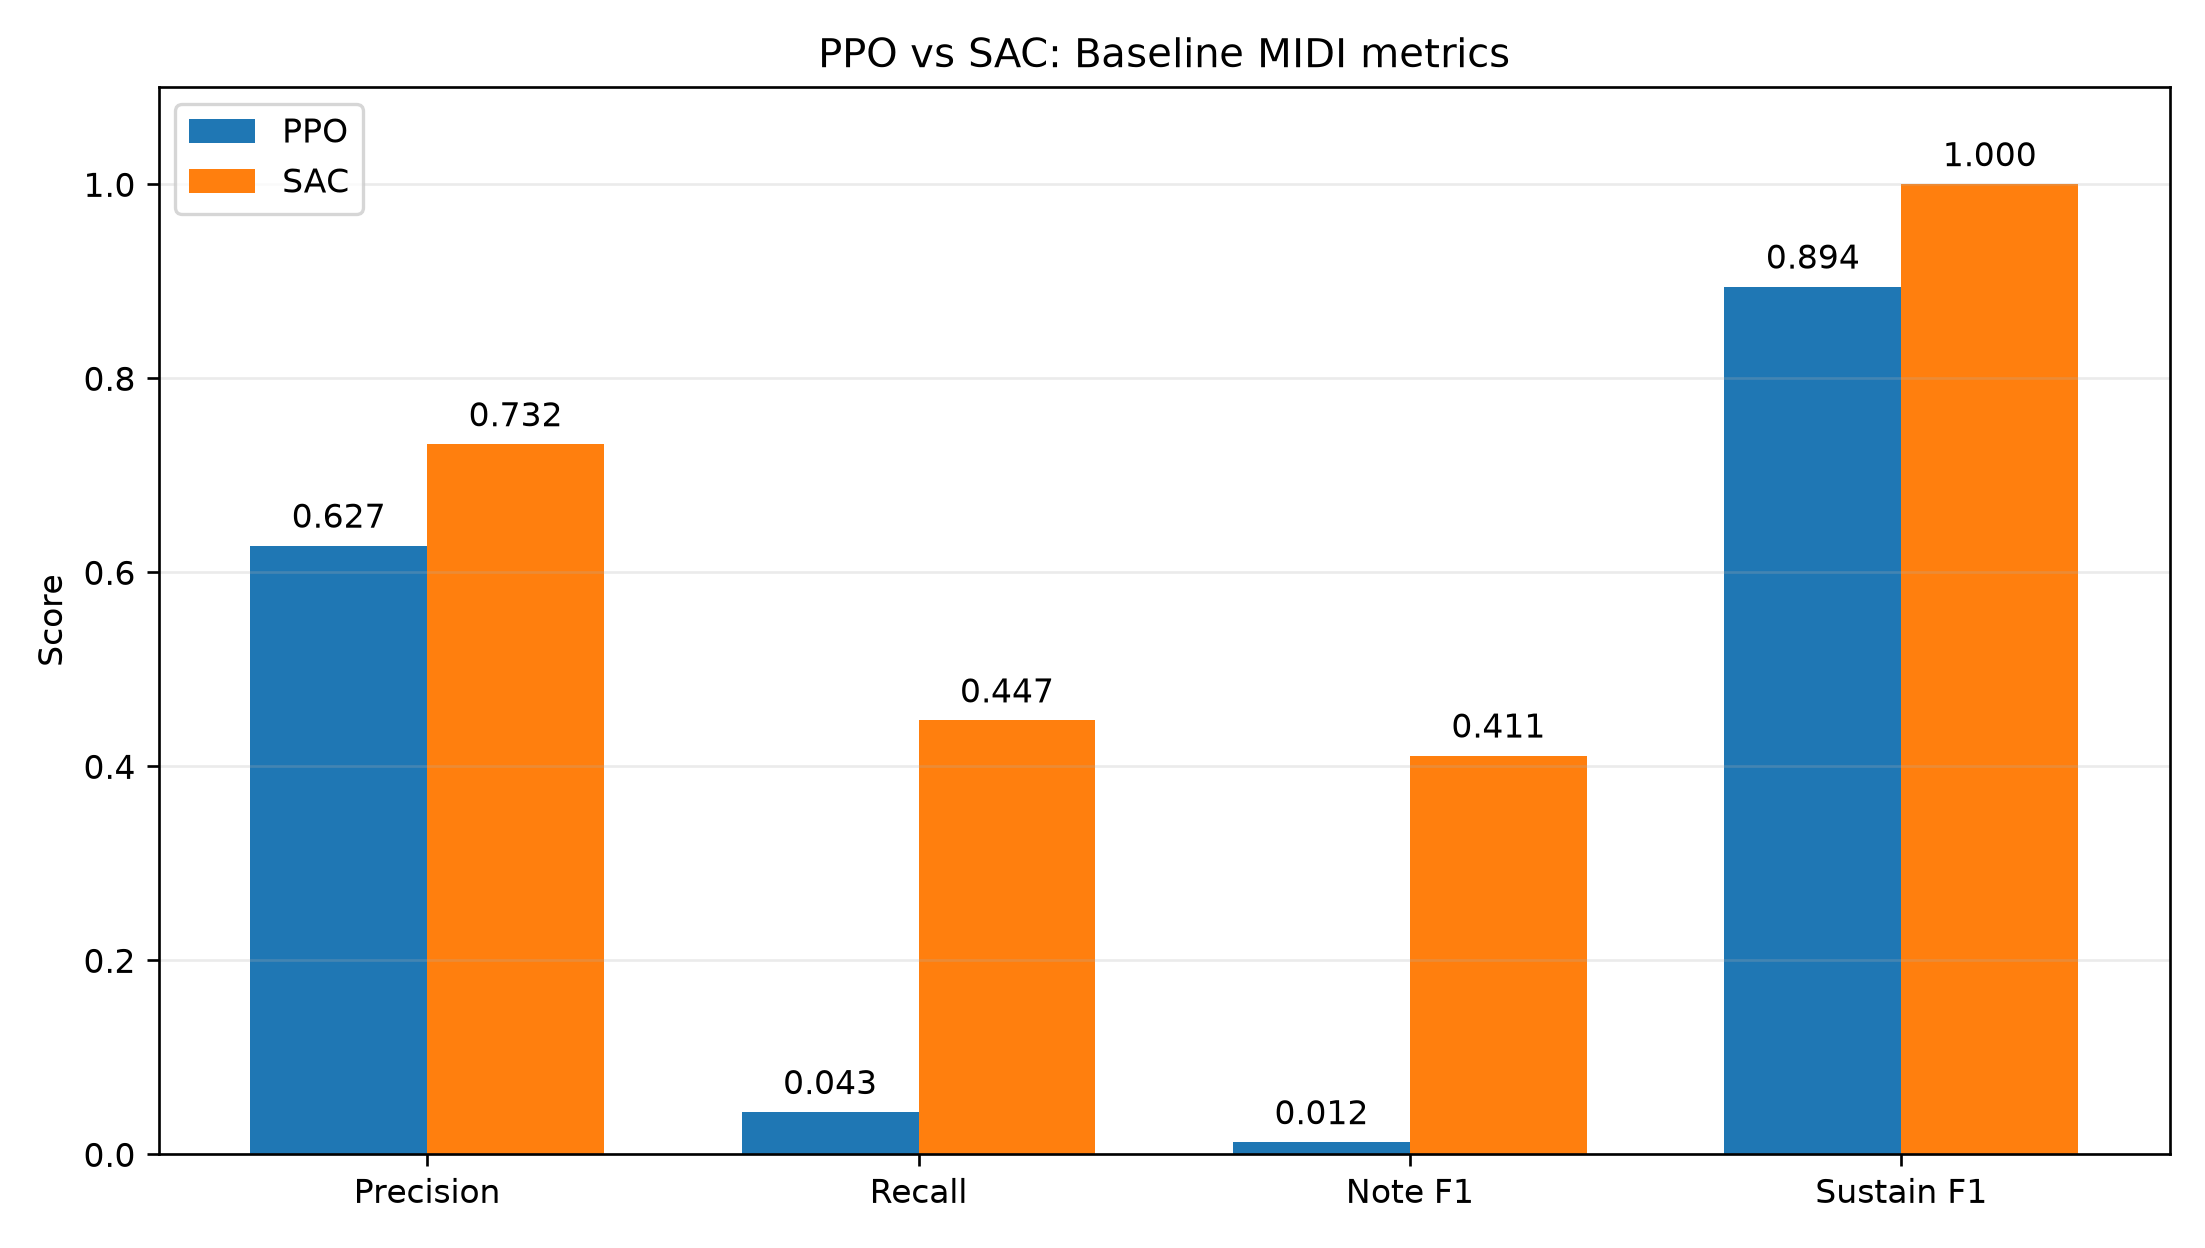
\includegraphics[width=0.88\textwidth]{images/baseline_metrics.png}
\caption{PPO 与 SAC 在基准场景中的音乐指标}
\label{fig:baseline-metrics}
\end{figure}

\subsection{多场景表现}

\begin{figure}[H]
\centering
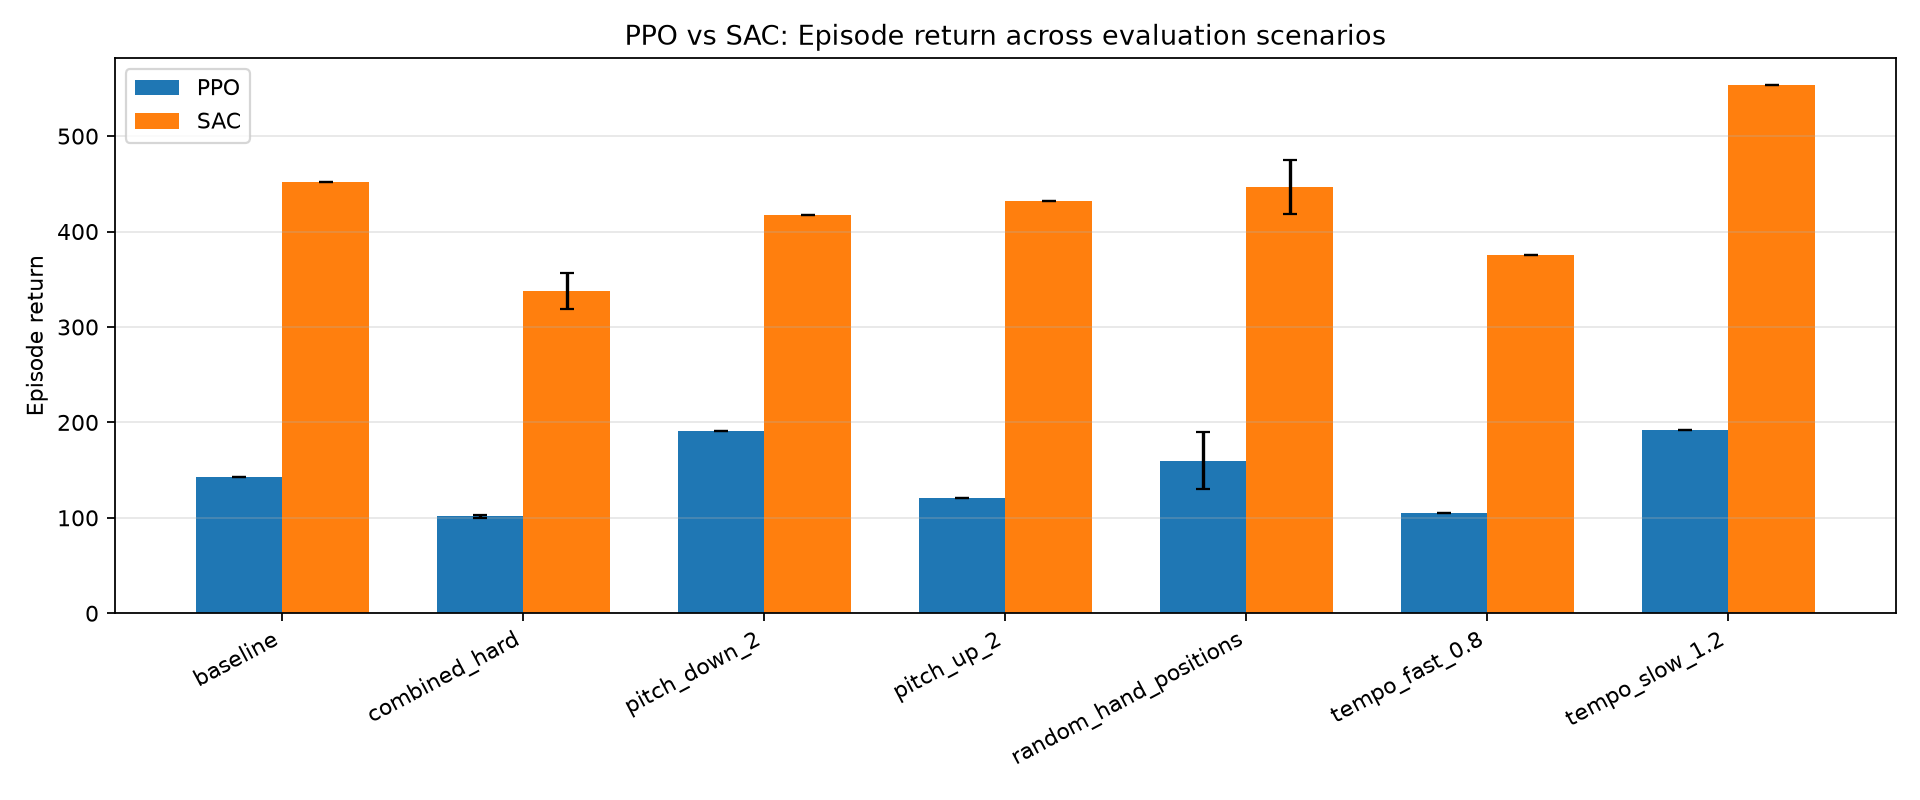
\includegraphics[width=\textwidth]{images/scenario_episode_return.png}
\caption{不同评估场景下的 episode return，误差线为三个评估回合的标准差}
\label{fig:scenario-return}
\end{figure}

慢速场景回合长度为 193，基准场景为 161，快速场景为 129，因此累计回报不能直接反映单位时间表现。图~\ref{fig:return-step} 给出了每步回报，SAC 在快速场景中的每步回报为 2.910，高于基准的 2.809。

\begin{figure}[H]
\centering
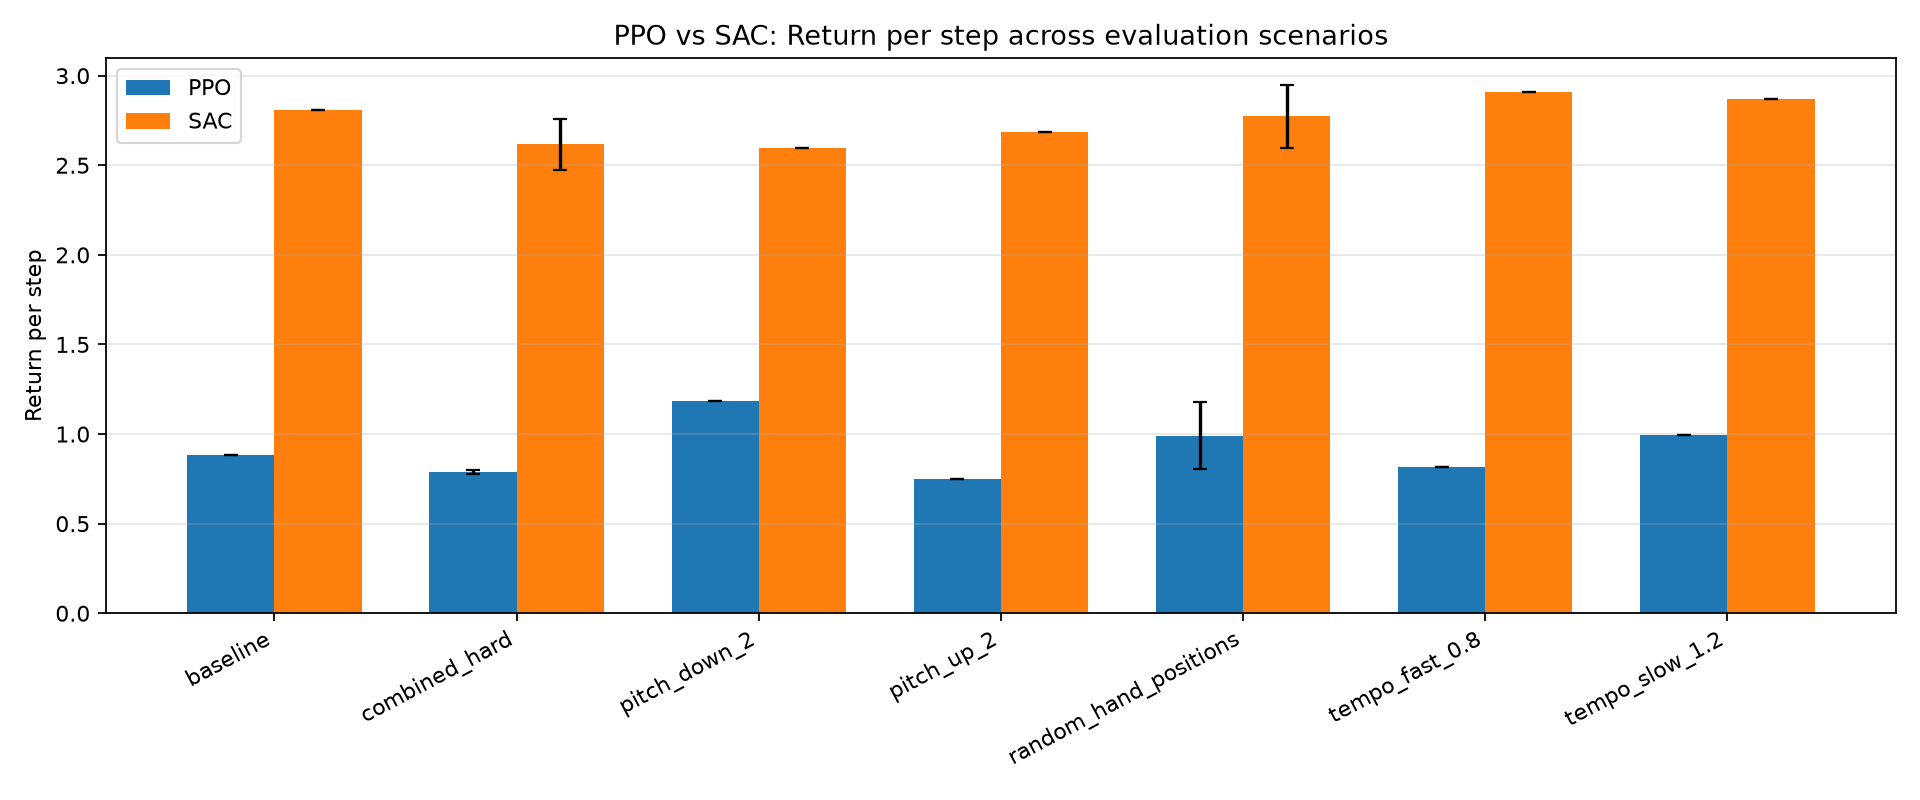
\includegraphics[width=\textwidth]{images/scenario_return_per_step.png}
\caption{不同评估场景下的每步回报}
\label{fig:return-step}
\end{figure}

\begin{figure}[H]
\centering
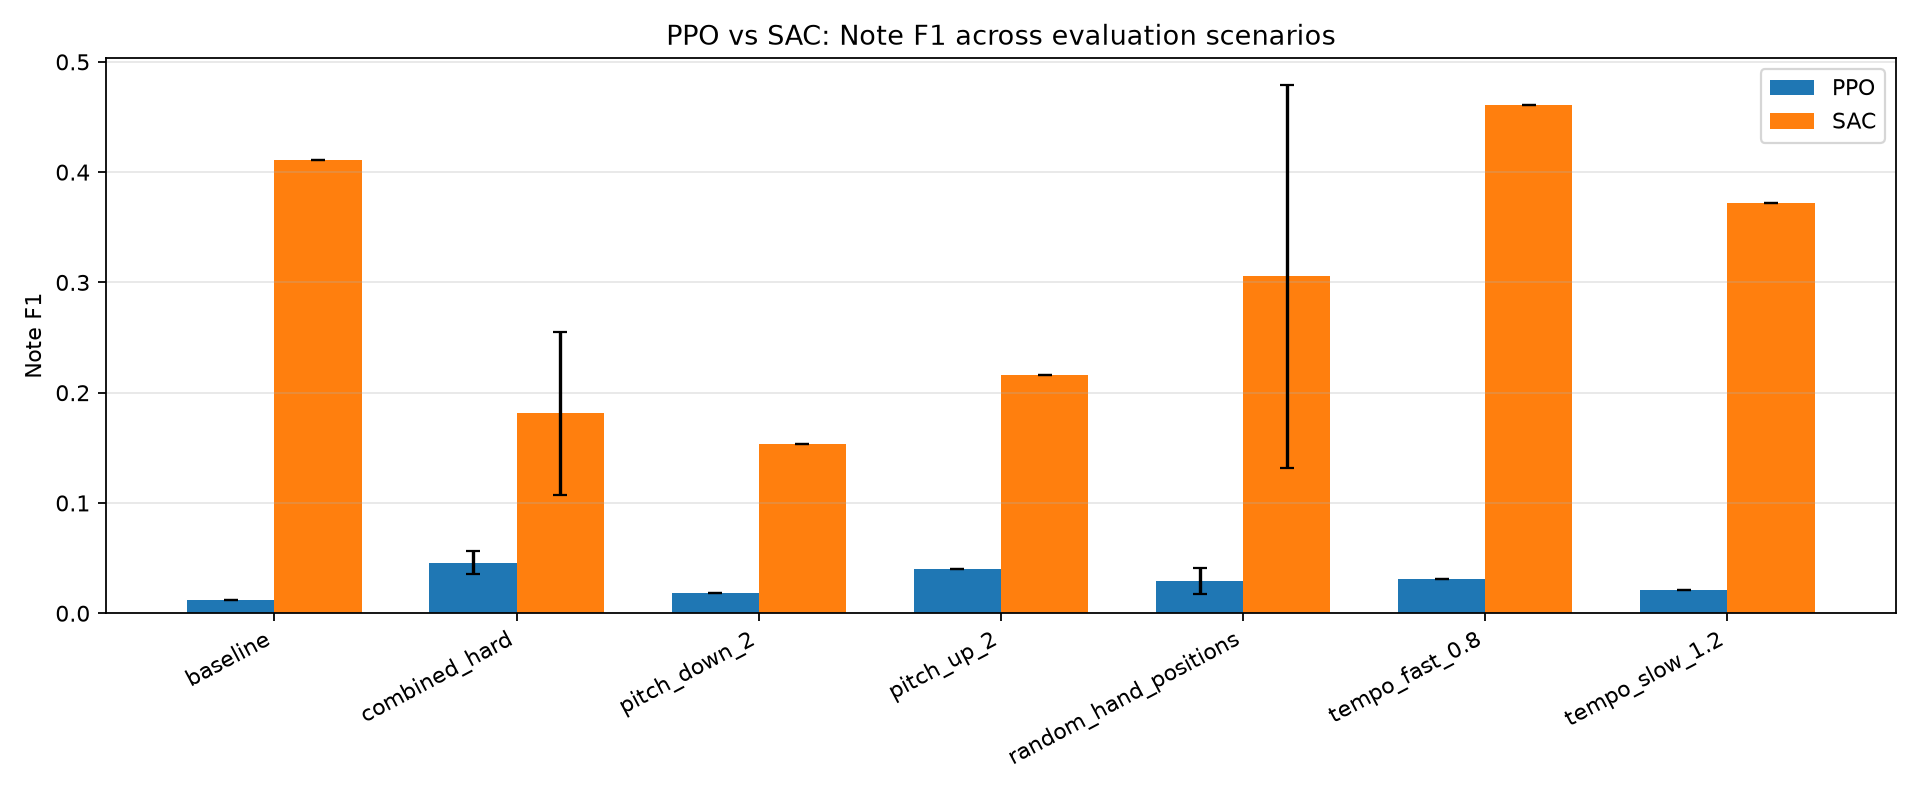
\includegraphics[width=\textwidth]{images/scenario_f1.png}
\caption{不同评估场景下的 Note F1（逐控制步按键激活 F1 的回合均值）}
\label{fig:scenario-f1}
\end{figure}

图~\ref{fig:scenario-f1} 显示所评估 SAC 模型在本次七个场景中的 Note F1 均高于所评估 PPO 模型。SAC 在快速场景取得最高值 0.460，在本轮评估中没有出现相对于基准场景的下降；降调后降至 0.153，随机手位场景的均值为 0.305、总体标准差为 0.174。这些结果表明当前 SAC 模型对音高变化和共同横向手位偏移较敏感，但样本量不足以用于统计推断。

\begin{landscape}
\begin{table}[H]
\centering
\scriptsize
\caption{多场景结果（三回合均值；$\pm$ 后为标准差）}
\begin{tabular}{llrrrrrr}
\toprule
算法 & 场景 & Return & Return/step & Precision & Recall & Note F1 & Sustain F1 \\
\midrule
PPO & baseline & 142.497 & 0.885 & 0.627 & 0.043 & 0.012 & 0.894 \\
SAC & baseline & 452.259 & 2.809 & 0.732 & 0.447 & 0.411 & 1.000 \\
PPO & tempo slow & 192.019 & 0.995 & 0.617 & 0.041 & 0.021 & 0.927 \\
SAC & tempo slow & 554.032 & 2.871 & 0.780 & 0.404 & 0.372 & 1.000 \\
PPO & tempo fast & 105.016 & 0.814 & 0.605 & 0.054 & 0.031 & 0.938 \\
SAC & tempo fast & 375.372 & 2.910 & 0.846 & 0.519 & 0.460 & 1.000 \\
PPO & pitch down & 191.096 & 1.187 & 0.571 & 0.043 & 0.019 & 0.907 \\
SAC & pitch down & 417.640 & 2.594 & 0.966 & 0.161 & 0.153 & 1.000 \\
PPO & pitch up & 120.389 & 0.748 & 0.735 & 0.050 & 0.040 & 0.882 \\
SAC & pitch up & 432.117 & 2.684 & 0.902 & 0.236 & 0.216 & 1.000 \\
PPO & random hands & $159.566\pm29.862$ & $0.991\pm0.185$ & $0.714\pm0.162$ & 0.043 & $0.029\pm0.012$ & $0.903\pm0.020$ \\
SAC & random hands & $446.535\pm28.466$ & $2.774\pm0.177$ & $0.761\pm0.107$ & $0.321\pm0.176$ & $0.305\pm0.174$ & 1.000 \\
PPO & combined hard & $101.569\pm1.429$ & $0.787\pm0.011$ & $0.782\pm0.028$ & $0.059\pm0.007$ & $0.046\pm0.011$ & $0.922\pm0.033$ \\
SAC & combined hard & $337.540\pm18.524$ & $2.617\pm0.144$ & $0.908\pm0.021$ & $0.198\pm0.068$ & $0.181\pm0.074$ & 1.000 \\
\bottomrule
\end{tabular}
\end{table}
\end{landscape}

\subsection{检查点扫描}

\begin{figure}[H]
\centering
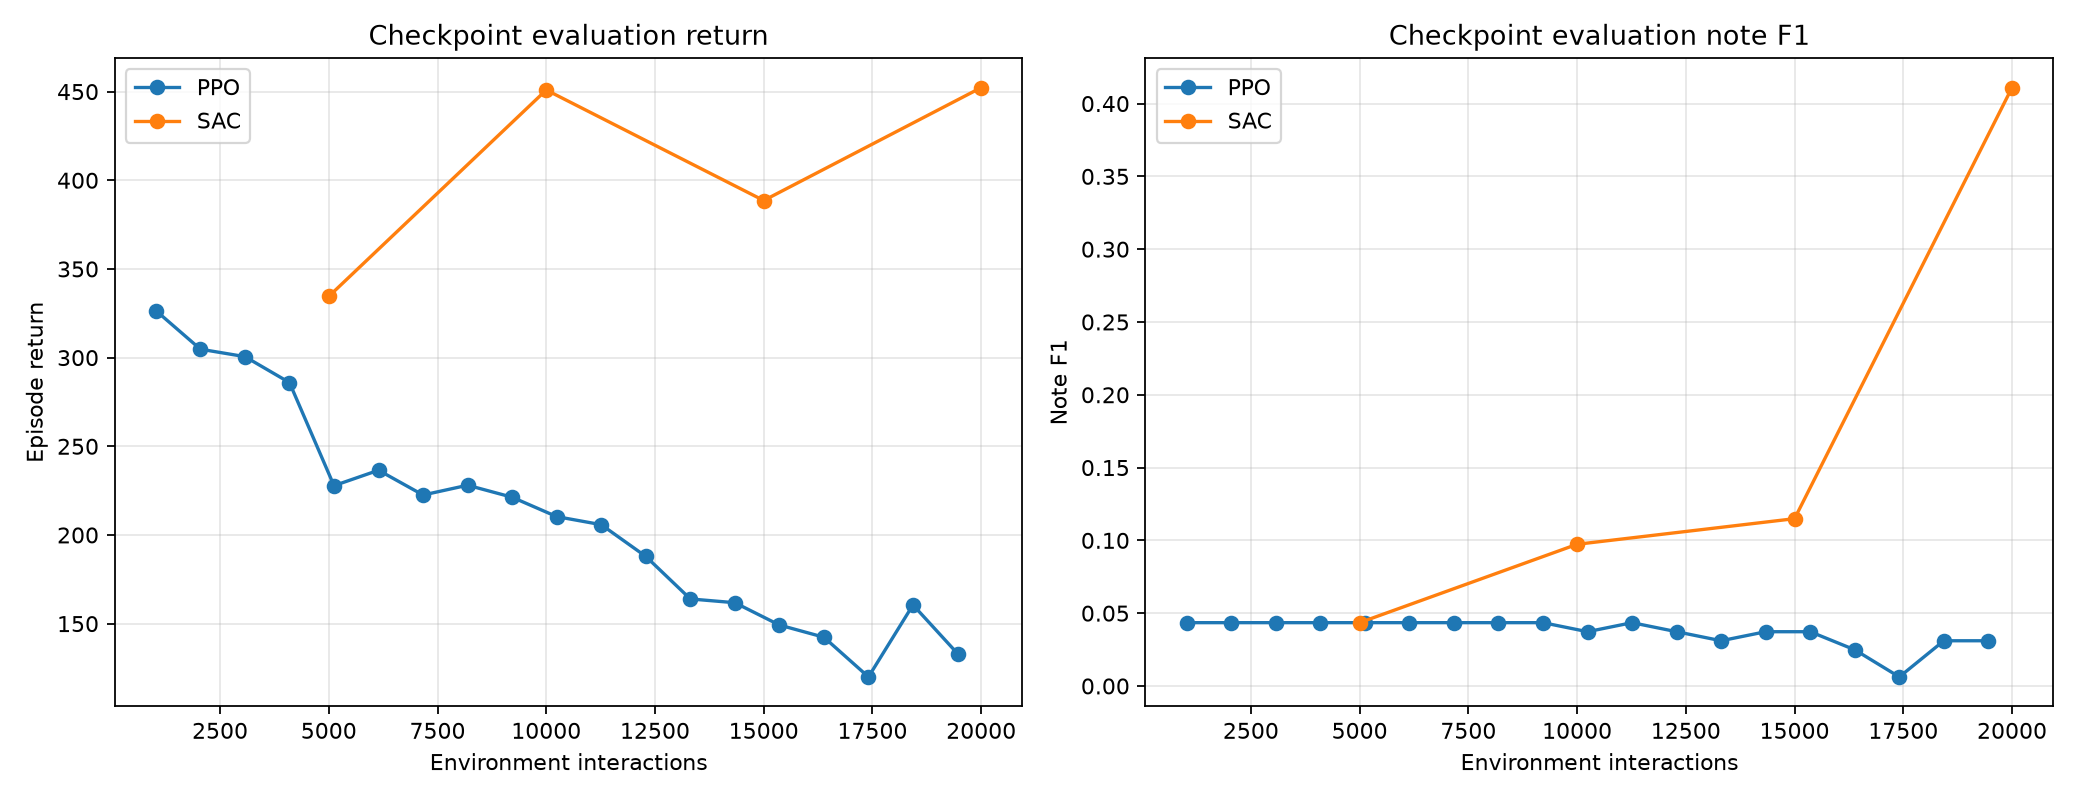
\includegraphics[width=\textwidth]{images/checkpoint_sweep.png}
\caption{PPO 与 SAC 检查点的回报和 Note F1}
\label{fig:checkpoint}
\end{figure}

在这个单训练种子中，PPO 的检查点回报总体随训练推进而下降：1,024 步检查点回报为 326.521，而另行评估的 20,224 步最终模型为 142.497。早期检查点 Note F1 约为 0.043，最终模型为 0.012。这说明当前这一次 PPO 训练在后期出现了评估性能退化；仅凭一次训练不能确定退化原因，也不能证明增加训练步数后一定无法恢复。

SAC 的 Note F1 从 5k 的 0.043 上升到 20k 的 0.411。虽然 15k 回报低于 10k，说明过程并非严格单调，但在本次扫描的四个检查点中，20k 同时取得最高回报和最高 Note F1。

\subsection{失败案例分析}

PPO 的第 25 百分位阈值为 0.0186。按“$F_1\leq$ 阈值”的规则，由于并列值存在，实际选中 7/21 个回合：基准场景三个回合、降调场景三个回合，以及随机手位 seed 20002。其共同特点是平均 Recall 很低，即只有少量控制步实现目标按键激活。环境原始回报是五项之和：按键、踏板、能量、指法和前臂碰撞奖励，因此较高回报不一定对应较高 Note F1。例如 PPO 在降调场景中的回报高于基准，但 Note F1 仍然接近 0。

SAC 的第 25 百分位阈值为 0.1576，同样由于阈值并列，实际选中 6/21 个回合：降调场景三个回合、随机手位 seed 20001，以及组合困难场景 seed 20001 和 20002。降调场景中平均 Precision 为 0.966，而平均 Recall 为 0.161，表明策略在多数控制步没有覆盖移调后的目标按键激活。随机手位与组合场景在三个种子之间出现较大差异，说明当前 SAC 策略对这种共同横向手位偏移较敏感。

\section{结果分析}

\subsection{当前结果中 SAC 表现更好的可能原因}

在约 20k 的较小交互预算下，SAC 的经验回放机制能够重复利用历史交互，而 PPO 只使用当前 rollout 进行更新。样本复用、双 Critic、目标网络和熵正则可能与 SAC 在本次实验中的较高结果有关，但本实验没有逐项消融，不能据此确定因果关系。

这并不意味着 SAC 在所有条件下必然优于 PPO。两种基线不仅算法不同，还使用不同训练种子、折扣系数、网络结构、观察预处理与训练框架，且每种算法只有一个训练种子。因此结论只能表述为“当前两套本机配置和约 20k 预算下，所评估 SAC 模型的数值高于所评估 PPO 模型”，不能视为算法总体优劣结论。

\subsection{回报与音乐准确率的差异}

实验中多次出现回报较高但 Note F1 较低的情况。环境每步回报是按键、踏板、能量、指法和前臂碰撞五项之和，而 Note F1 只比较目标按键与实际按键的二值激活。策略可以从其他奖励项获得分数，因此累计回报与 Note F1 不必同步变化。模型选择至少应同时考虑：
\begin{itemize}
  \item episode return；
  \item return per step；
  \item note Precision、Recall 和 F1；
  \item sustain F1；
  \item 不同随机初态下的均值和方差。
\end{itemize}

\section{实验说明}

\begin{enumerate}
  \item PPO 和 SAC 均只有一个训练种子，不能进行统计显著性推断；
  \item 固定手位场景的三个评估种子产生相同轨迹，不能当作三个独立样本；
  \item PPO 与 SAC 的训练种子、折扣因子、网络结构和训练框架不同；PPO 使用观察/训练奖励归一化，SAC 不使用该归一化且观察还额外包含上一动作和奖励，因此不是严格控制变量的算法消融；
  \item 本阶段复用已有约 20k 训练产物，重点是补齐评估闭环，而非重新训练多组模型；
  \item 训练步数相对于高维双手钢琴任务仍然较少。
\end{enumerate}

\end{document}
